\documentclass[11pt]{article}

\usepackage[margin=.82in]{geometry}
\usepackage[T1]{fontenc}
\usepackage{libertinus}
\usepackage{microtype}
\usepackage{mathtools,amssymb,amsthm}
\usepackage{booktabs}
\usepackage{enumitem}
\usepackage{titlesec}
\usepackage{fancyhdr}
\usepackage{xcolor}
\usepackage{tikz}
\usetikzlibrary{arrows.meta,positioning,fit}
\usepackage{pgfplots}
\usepgfplotslibrary{groupplots}
\pgfplotsset{compat=1.18}
\usepackage[hidelinks]{hyperref}
\usepackage{orcidlink}

\definecolor{ink}{HTML}{263238}
\definecolor{blue}{HTML}{356A8A}
\definecolor{gold}{HTML}{C28A35}
\definecolor{pale}{HTML}{EDF3F6}
\colorlet{orcidlogocol}{black}
\hypersetup{
  pdftitle={Behavioral Embeddings and Propensity Neighborhoods for Program Recommendation},
  pdfauthor={J. R. Landers},
  pdfsubject={Behavioral embeddings, nested propensity neighborhoods, calibration, and energy program recommendation},
  pdfkeywords={recommender systems, energy programs, propensity models, behavioral embeddings, customer neighborhoods, calibration}
}

\setlength{\parindent}{1.0em}
\setlength{\parskip}{0pt}
\linespread{0.965}
\setlength{\abovedisplayskip}{4pt plus 1pt minus 1pt}
\setlength{\belowdisplayskip}{4pt plus 1pt minus 1pt}
\setlength{\textfloatsep}{6pt plus 2pt minus 2pt}
\setlength{\floatsep}{5pt plus 2pt minus 2pt}
\setlist{nosep,leftmargin=1.4em}
\setcounter{secnumdepth}{2}
\titleformat{\section}{\large\bfseries\scshape}{\thesection}{0.65em}{}
\titleformat{\subsection}{\normalsize\bfseries}{\thesubsection}{0.6em}{}
\titlespacing*{\section}{0pt}{.9ex plus .2ex}{.35ex}
\titlespacing*{\subsection}{0pt}{.7ex plus .2ex}{.25ex}

\newtheoremstyle{noteplain}{.45ex}{.45ex}{\itshape}{}{\bfseries}{.}{.45em}{}
\theoremstyle{noteplain}
\newtheorem{theorem}{Theorem}
\newtheorem{proposition}[theorem]{Proposition}
\newtheorem{corollary}[theorem]{Corollary}
\theoremstyle{definition}
\newtheorem{remark}[theorem]{Remark}

\makeatletter
\renewenvironment{proof}[1][\proofname]{\par
  \pushQED{\qed}%
  \normalfont \topsep5\p@\@plus5\p@\relax
  \trivlist
  \item[\hskip\labelsep\bfseries #1\@addpunct{.}]\ignorespaces
}{%
  \popQED\endtrivlist\@endpefalse
}
\makeatother

\newcommand{\E}{\mathbb E}
\newcommand{\cA}{\mathcal A}
\newcommand{\cN}{\mathcal N}
\newcommand{\argmax}{\operatorname*{arg\,max}}
\newcommand{\argmin}{\operatorname*{arg\,min}}

\pagestyle{fancy}
\fancyhf{}
\fancyhead[L]{\footnotesize\scshape Propensity Neighborhoods}
\fancyhead[R]{\footnotesize J. R. Landers}
\fancyfoot[C]{\footnotesize\thepage}
\renewcommand{\headrulewidth}{0.35pt}
\setlength{\headheight}{14pt}

\begin{document}

\begin{center}
  {\LARGE\bfseries Behavioral Embeddings and Propensity Neighborhoods for Program Recommendation\par}
  \vspace{0.7em}
  {\large J. R. Landers\,\orcidlink{0000-0003-1872-6179}\par}
  \vspace{0.12em}
  {\small September 2026}
\end{center}

\vspace{0.05em}
\section{Setting}

Suppose a utility can estimate every eligible program's enrollment propensity for every customer. A direct recommender can mask ineligible programs and choose the largest fitted propensity, but even a strong model may retain local patterns of overprediction and underprediction. The question is whether similar historical customers provide enough evidence to correct those remaining errors before a program is chosen.

The proposed recommender first converts behavioral history into customer coordinates and uses them to estimate one propensity score for every program. It then retrieves historical customers with similar representations or propensity profiles and averages their out-of-fold model residuals to calibrate the target customer's scores. Adding coordinate blocks makes these fixed-radius neighborhoods more specific but also thinner, so the method must stop when a better local match no longer compensates for the loss of peer support.

These pieces form an operational workflow: filter eligible programs, learn the behavioral representation, score the propensity row, retrieve nested peers, select a support-aware refinement depth, and then calibrate, rank, or abstain. The workflow combines the primary predictive model, the local correction, and the theorem's decision certificate in one implementable sequence.

The theory and experiments organized around this workflow yield three connected conclusions:

\begin{center}
\emph{Behavioral embeddings provide the largest empirical gain by creating customer coordinates that preserve future propensity similarity. Operational peer-mean neighborhood calibration adds a small but consistent improvement in propensity RMSE, without a detectable improvement in the winning recommendation. The refinement-frontier theorem and its operational corollaries provide finite-sample guarantees for latent propensities under a valid residual band and marginal guarantees for realized outcomes under exchangeability.}
\end{center}

\section{From behavior to a propensity matrix}

Let $x_1,\ldots,x_N$ be $N$ customers and let $\cA=\{a_1,\ldots,a_K\}$ be a common catalog of $K$ programs. Thus $i\in\{1,\ldots,N\}$ indexes customers and $j\in\{1,\ldots,K\}$ indexes programs. Eligibility is applied before an individual recommendation, giving the feasible subset $\cA(x)\subseteq\cA$ for target customer $x$. For any customer $x$ and program $a$, define the true enrollment propensity
\[
 p_a(x)=\Pr(\text{$x$ enrolls in program $a$})\in[0,1].
\]
Collect the $K$ catalog propensities into the row vector $p(x)=(p_{a_j}(x):j=1,\ldots,K)\in[0,1]^K$. The true customer-by-program matrix is $P=(p_{a_j}(x_i))\in[0,1]^{N\times K}$. A fitted model supplies an estimate $\widetilde p_a(x)$ of each probability and hence the fitted matrix
\[
\widetilde P=
\begin{bmatrix}
\widetilde p_{a_1}(x_1)&\widetilde p_{a_2}(x_1)&\cdots&\widetilde p_{a_K}(x_1)\\
\widetilde p_{a_1}(x_2)&\widetilde p_{a_2}(x_2)&\cdots&\widetilde p_{a_K}(x_2)\\
\vdots&\vdots&\ddots&\vdots\\
\widetilde p_{a_1}(x_N)&\widetilde p_{a_2}(x_N)&\cdots&\widetilde p_{a_K}(x_N)
\end{bmatrix}\in[0,1]^{N\times K}.
\]
Thus the row $\widetilde p(x)=(\widetilde p_{a_j}(x):j=1,\ldots,K)\in[0,1]^K$ is a fitted propensity vector. A tilde marks a fitted quantity throughout. The base recommender masks ineligible columns and ranks the remaining entries:
\begin{equation}\label{eq:base-rank}
 \widetilde a(x)\in\argmax_{a\in\cA(x)}\widetilde p_a(x).
\end{equation}

\subsection{A behavioral embedding}

Customer attributes need not be the only coordinates. Let $H=(H_{i\ell})\in\mathbb R^{N\times J}$ record pre-decision behavior over $J$ items or events, where $H_{i\ell}$ is customer $i$'s bounded engagement with item or event $\ell\in\{1,\ldots,J\}$. Choose an embedding dimension $D\leq\min\{N,J\}$. A rank-$D$ factorization,
\[
 H\approx U_D\Sigma_DV_D^\top,
 \qquad z(x_i)=(U_D\Sigma_D)_{i\cdot}\in\mathbb R^D,
\]
where $U_D\in\mathbb R^{N\times D}$ and $V_D\in\mathbb R^{J\times D}$ contain customer and item directions, $\Sigma_D\in\mathbb R^{D\times D}$ contains their singular values, ${}^\top$ denotes transpose, and $(\cdot)_{i\cdot}$ selects row $i$. This maps a long behavioral history to a $D$-coordinate customer embedding $z(x_i)$, following the matrix-factorization tradition in collaborative filtering \cite{koren}. Modern sequential recommenders learn richer behavioral representations with causal or bidirectional self-attention \cite{sasrec,bert4rec}, while recent generative-retrieval systems encode interaction histories and items as semantic tokens \cite{tiger}. The factorization here is deliberately transparent rather than architecture-specific, and it is learned from history only. If $s(x)$ denotes the vector of ordinary premise and customer attributes, a program model $f_a$ takes the form
\begin{equation}\label{eq:prop-model}
 \widetilde p_a(x)=f_a\bigl(s(x),z(x)\bigr),\qquad a\in\cA.
\end{equation}
Any supervised or unsupervised embedding may replace the factorization; what matters below is whether distance in its coordinates preserves future propensity similarity.

This representation is the primary predictive layer. The neighborhood method introduced next is deliberately downstream: it asks whether historical customers close in the learned geometry can correct residual errors left by the propensity model.

\begin{center}

\begin{tikzpicture}[
  node distance=3.5mm,
  box/.style={draw=ink,rounded corners=1.5pt,fill=pale,align=center,minimum height=7.2mm,text width=27mm,font=\small},
  arrow/.style={-{Latex[length=2mm]},thick,draw=blue}
]
\node[box] (history) {attributes $s(x)$\\history $H_{i\cdot}$};
\node[box,right=of history] (embed) {embedding\\$z(x)$};
\node[box,right=of embed,text width=32mm] (scores) {program models\\$\widetilde p(x)$, row of $\widetilde P$};
\node[box,right=of scores,text width=31mm] (near) {nested neighbors\\match $+$ support};
\node[box,right=of near,text width=28mm] (decision) {calibrate, rank,\\or abstain};
\draw[arrow] (history)--(embed);
\draw[arrow] (embed)--(scores);
\draw[arrow] (scores)--(near);
\draw[arrow] (near)--(decision);
\end{tikzpicture}
\refstepcounter{figure}
\parbox{.94\linewidth}{\small\textbf{Figure \thefigure.} The recommender first learns a representation and a propensity row. Neighborhoods add a local evidence layer around that row.}
\label{fig:pipeline}
\end{center}

\section{Nested neighborhoods}

Once the base propensity row exists, the remaining question is how much detail a local correction can safely use. Let $x$ denote a target customer and let $x_1,\ldots,x_n$ denote $n$ historical reference customers, renumbered for convenience from the larger customer population. Choose a positive integer $M$ and order the available representation into $M$ blocks. Blocks may contain static attributes, groups of embedding coordinates, or groups of fitted propensity coordinates. Let $d_m(x,x')\geq0$ be the cumulative distance after the first $m$ blocks and require
\[
 d_{m+1}(x,x')\geq d_m(x,x'),\qquad m=1,\ldots,M-1.
\]
Equivalently, set $\delta_1(x,x')=d_1(x,x')$ and $\delta_j(x,x')=d_j(x,x')-d_{j-1}(x,x')\geq0$ for $j\geq2$, so that $d_m(x,x')=\sum_{j=1}^m\delta_j(x,x')$. This includes cumulative Euclidean, block-additive, and maximum-coordinate distances. For a fixed radius $r\geq0$, set
\[
 \cN_m(x;r)=\{i\in\{1,\ldots,n\}:d_m(x,x_i)\leq r\},
 \qquad n_m=|\cN_m(x;r)|.
\]
Only nonempty levels are considered.

Local averaging over nearby profiles belongs to the classical nonparametric-regression tradition \cite{stone}. More recent local-calibration methods likewise assess reliability around similar predictions in a pretrained feature space \cite{luo}. The construction here differs by calibrating an entire program-indexed residual vector and nesting fixed-radius neighborhoods by declared feature blocks, which makes the support spent by each refinement explicit.

\begin{proposition}[More detail leaves fewer peers]\label{prop:thin}
For $m=1,\ldots,M-1$,
\[
 \cN_{m+1}(x;r)\subseteq\cN_m(x;r),\qquad n_{m+1}\leq n_m.
\]
\end{proposition}

\begin{proof}
Because $\delta_{m+1}\geq0$, $d_{m+1}(x,x')\geq d_m(x,x')$. A customer within radius $r$ after block $m+1$ was therefore within radius $r$ after block $m$.
\end{proof}

The refinement cost is exact: each added block can spend peer support. To describe its benefit, let $g(x)=(g_a(x):a\in\cA)\in\mathbb R^K$ be any catalog-indexed target quantity whose local homogeneity matters and define
\[
 \varepsilon_m^g(x)=\max_{i\in\cN_m(x;r)}\|g(x_i)-g(x)\|_\infty,
\]
where $\|v\|_\infty=\max_{a\in\cA}|v_a|$; for a target-specific certificate, the maximum may be restricted to $a\in\cA(x)$. For direct peer averaging take $g=p$. For residual calibration take
\[
 g(x)=\rho(x):=p(x)-\widetilde p(x),
\]
the vector of errors remaining after the base propensity model; its program-$a$ coordinate is $\rho_a(x)=p_a(x)-\widetilde p_a(x)$.

\begin{proposition}[Refinement improves worst-case local similarity]\label{prop:mismatch}
If $\cN_{m+1}(x;r)$ is nonempty, then
\[
 \varepsilon_{m+1}^g(x)\leq\varepsilon_m^g(x).
\]
\end{proposition}

\begin{proof}
By Proposition~\ref{prop:thin}, the later neighborhood is a subset of the earlier one. The maximum of the same nonnegative function over a subset cannot increase.
\end{proof}

The fitted propensity matrix gives a particularly compact geometry. Full-row matching uses
\[
 d_p(x,x_i)=\|\widetilde p(x)-\widetilde p(x_i)\|_\infty.
\]
When calibrating a particular program $a$, a leave-one-program-out alternative uses
\[
 d_{-a}(x,x_i)=\max_{b\in\cA\setminus\{a\}}
 |\widetilde p_b(x)-\widetilde p_b(x_i)|.
\]
Both are available once $\widetilde P$ has been scored. Progressive groups of propensity coordinates also satisfy Proposition~\ref{prop:thin}. The two propositions now establish the geometric tradeoff: refinement cannot worsen the worst remaining match, but it can only preserve or reduce peer support. The next section converts that tradeoff into a statistical guarantee.

\section{The refinement frontier}

We now use local residual homogeneity to bound the error of the final program choice. For reference customer $i\in\{1,\ldots,n\}$ and program $a\in\cA(x)$, let $Y_{ia}\in[0,B]$, where $B>0$, be a bounded calibration outcome satisfying $\E[Y_{ia}\mid x_i]=p_a(x_i)$. For binary enrollment, $B=1$. Historical fitted scores $\widetilde p_a(x_i)$ are computed out of fold or on a separate fitting sample. At level $m$, use the peers' mean residual to correct the target score:
\begin{equation}\label{eq:residual}
 \widehat p_{a,m}(x)=\widetilde p_a(x)
 +\frac{1}{n_m}\sum_{i\in\cN_m(x;r)}
 \bigl(Y_{ia}-\widetilde p_a(x_i)\bigr),
 \qquad
 \widehat a_m\in\argmax_{a\in\cA(x)}\widehat p_{a,m}(x).
\end{equation}
The estimate may be clipped to $[0,1]$ coordinatewise. Let $a^*\in\argmax_{a\in\cA(x)}p_a(x)$ be a true best eligible program, let $K_x=|\cA(x)|$ be the number of eligible programs, and write $\varepsilon_m^\rho(x)$ for the residual mismatch defined above.

\begin{theorem}[Residual refinement frontier]\label{thm:frontier}
Suppose that, conditional on the customer profiles, the calibration outcomes $\{Y_{ia}:i=1,\ldots,n\}$ are independent for each $a$, and that the neighborhoods are fixed independently of these outcomes. For a prespecified level $m$ with $n_m\geq1$ and confidence parameter $\alpha\in(0,1)$, with probability at least $1-\alpha$,
\[
 p_{a^*}(x)-p_{\widehat a_m}(x)
 \leq 2b_m(x),\qquad
 b_m(x)=\varepsilon_m^\rho(x)
 +B\sqrt{\frac{\log(2K_x/\alpha)}{2n_m}}.
\]
If one of $M$ levels is selected using the same calibration outcomes, replace $K_x$ by $K_xM$.
\end{theorem}

\begin{proof}
Let $\bar\rho_{a,m}(x)=n_m^{-1}\sum_{i\in\cN_m(x;r)}\rho_a(x_i)$ be the peers' mean true residual. Taking conditional expectations in \eqref{eq:residual} gives $\widetilde p_a(x)+\bar\rho_{a,m}(x)$. Since $p_a(x)=\widetilde p_a(x)+\rho_a(x)$,
\[
 |\bar\rho_{a,m}(x)-\rho_a(x)|\leq\varepsilon_m^\rho(x).
\]
Hoeffding's inequality \cite{hoeffding} and a union bound over the $K_x$ eligible programs bound the deviation of each empirical mean residual from $\bar\rho_{a,m}(x)$ by
$q_m=B\sqrt{\log(2K_x/\alpha)/(2n_m)}$. Thus
$|\widehat p_{a,m}(x)-p_a(x)|\leq b_m(x)$ simultaneously in $a$. Because $\widehat a_m$ maximizes the fitted values,
\[
 p_{a^*}(x)-p_{\widehat a_m}(x)
 \leq[p_{a^*}(x)-\widehat p_{a^*,m}(x)]
 +[\widehat p_{\widehat a_m,m}(x)-p_{\widehat a_m}(x)]
 \leq2b_m(x).
\]
A second union bound over $M$ levels proves the adaptive statement.
\end{proof}

The two terms move in opposite directions. Proposition~\ref{prop:mismatch} makes the residual mismatch nonincreasing; Proposition~\ref{prop:thin} makes the uncertainty term nondecreasing. Let $\widehat\varepsilon_m^\rho(x)\geq0$ denote an estimate of $\varepsilon_m^\rho(x)$ obtained from separate validation data or cross-fitted residuals. A literal finite-sample certificate uses an upper confidence estimate; a validation estimate gives the corresponding tuning rule. The customer-specific choice is
\begin{equation}\label{eq:rule}
 \widehat m(x)\in\argmin_{1\leq m\leq M}
 \left\{\widehat\varepsilon_m^\rho(x)
 +B\sqrt{\frac{\log(2K_xM/\alpha)}{2n_m}}\right\}.
\end{equation}
This minimizing level gives the title its operational meaning: the last useful feature block is the last refinement whose gain in local match quality is worth the peer support it spends.

The true mismatch in \eqref{eq:rule} is not generally observed for a new customer. A separate residual model makes the frontier operational without pretending otherwise. Let $\widehat\rho(x)$ be trained away from the reference and target outcomes, let
\[
 R_i=Y_i-\widetilde p(x_i),\qquad
 c_m(x)=\lambda_m\frac{1}{n_m}\sum_{i\in\cN_m(x;r)}R_i,
 \qquad \lambda_m\in[0,1],
\]
and include a level $m=0$ with $c_0(x)=0$. Two observable discrepancies are
\begin{align*}
 D_m^{\mathrm{mean}}(x)
 &=\|\widehat\rho(x)-c_m(x)\|_\infty,\\
 D_m^{\max}(x)
 &=\lambda_m\max_{i\in\cN_m(x;r)}
   \|\widehat\rho(x)-R_i\|_\infty
   +(1-\lambda_m)\|\widehat\rho(x)\|_\infty.
\end{align*}
Convexity gives $D_m^{\mathrm{mean}}(x)\leq D_m^{\max}(x)$. The second expression retains the theorem's worst-neighbor form; the first exploits the fact that the implemented correction is specifically a peer mean.
For $m=0$, set both discrepancies to $\|\widehat\rho(x)\|_\infty$.

\begin{corollary}[Operational peer-mean frontier]\label{cor:operational}
Suppose an independently constructed simultaneous band satisfies
\[
 \Pr\!\left\{\|\rho(x)-\widehat\rho(x)\|_\infty\leq\eta(x)\right\}
 \geq1-\delta.
\]
Choose $\widehat m(x)$ by minimizing either observable discrepancy over the available levels, including $m=0$, without using $p(x)$. Then, with probability at least $1-\delta$,
\[
 \|p(x)-[\widetilde p(x)+c_{\widehat m}(x)]\|_\infty
 \leq \eta(x)+D_{\widehat m}^{\mathrm{mean}}(x)
 \leq \eta(x)+D_{\widehat m}^{\max}(x),
\]
and the selected program has propensity regret at most twice the corresponding right-hand side.
\end{corollary}

\begin{proof}
The first inequality is the triangle inequality applied to
$\rho(x)-c_{\widehat m}(x)=[\rho(x)-\widehat\rho(x)]+[\widehat\rho(x)-c_{\widehat m}(x)]$.
The second follows from convexity, and the regret step is the same two-error argument used in Theorem~\ref{thm:frontier}.
\end{proof}

Corollary~\ref{cor:operational} is a latent-propensity statement only when the stated band covers the latent residual $\rho(x)$. Ordinary split conformal calibration of observed outcomes does not, by itself, supply distribution-free pointwise coverage of a conditional mean. It does give a distinct operational guarantee. Freeze the entire peer-retrieval, level-selection, and correction algorithm before an independent calibration split; let $\widehat p^{\mathrm{op}}(x)$ denote its output and set
\[
 S_i=\|Y_i-\widehat p^{\mathrm{op}}(x_i)\|_\infty.
\]
If $q_{1-\alpha}$ is the split-conformal quantile with the standard finite-sample correction, exchangeability of the calibration users and a future user gives
\begin{equation}\label{eq:conformal-operational}
 \Pr\!\left\{
 \|Y-\widehat p^{\mathrm{op}}(X)\|_\infty\leq q_{1-\alpha}
 \right\}\geq1-\alpha,
\end{equation}
and realized-outcome regret is at most $2q_{1-\alpha}$ on that event \cite{shafer}. This coverage is finite-sample and marginal over a future exchangeable user; it is not conditional coverage of $p(x)$.

\begin{remark}[Known propensity coordinates]\label{rem:known}
Some coordinates need no residual model. If current enrollment or a deterministic eligibility state implies $p_a(x)=1$, then $\rho_a(x)=1-\widetilde p_a(x)$ is known at recommendation time; similarly, $p_a(x)=0$ gives $\rho_a(x)=-\widetilde p_a(x)$. A coordinatewise version of Corollary~\ref{cor:operational} sets the uncertainty radius to zero on these coordinates and retains a residual band only for the unknown coordinates. Thus partial knowledge can make the operational certificate strictly sharper.
\end{remark}

\begin{corollary}[A confident recommendation]\label{cor:margin}
Assume $K_x\geq2$. On the event in Theorem~\ref{thm:frontier}, let $\widehat a_m$ have empirical lead
\[
 \Delta_m(x)=\widehat p_{\widehat a_m,m}(x)
 -\max_{a\in\cA(x)\setminus\{\widehat a_m\}}\widehat p_{a,m}(x).
\]
If $\Delta_m(x)>2b_m(x)$, then $\widehat a_m$ is the unique true best program.
\end{corollary}

\begin{proof}
Every true propensity lies within $b_m$ of its estimate. An empirical lead exceeding $2b_m$ therefore remains positive after both scores move by their largest permitted errors.
\end{proof}

This result is related to, but distinct from, the broader calibration literature. Accurate modern predictors can still return unreliable probabilities, motivating global post-processing methods such as temperature scaling \cite{guo}; learned-space methods make that assessment local \cite{luo}; and recent distribution-free work seeks group-conditional and multicalibrated guarantees \cite{venn}. The present theorem instead controls the regret of the selected program and makes the guarantee depend explicitly on neighborhood mismatch and peer support.

Shrinkage is often useful in implementation. Multiplying the residual correction in \eqref{eq:residual} by $\lambda\in[0,1]$ changes the uniform error term to at most
\[
 (1-\lambda)\|\rho(x)\|_\infty
 +\lambda\varepsilon_m^\rho(x)+\lambda B\sqrt{\frac{\log(2K_x/\alpha)}{2n_m}}.
\]
Cross-validation can select $\lambda$ before the test period. Corollary~\ref{cor:margin} then turns the bound into a practical gate: rerank when local evidence clears the top-two margin, otherwise retain the base choice or mark it low confidence.

\section{A recommender workflow}

The three claims fit into a six-step operating loop: learn a useful representation, add local calibration only where it is supported, and use the guarantee to govern refinement and recommendation. Its separation of candidate generation from scoring follows the retrieve-and-rank pattern used in large-scale recommenders \cite{covington}, while the neighborhood and certificate layers determine whether local evidence should modify the ranker. Each step has an operational object and, where relevant, a formal guarantee.

Within the energy domain, collaborative-filtering systems have recommended retail electricity plans from appliance and consumption patterns \cite{zhangplan}, while smart-meter models have targeted customers for energy-efficiency programs \cite{liang}. The workflow below extends that line by joining behavioral representation and program scoring to local residual calibration and an explicit finite-sample decision gate.

\begin{enumerate}[label=\textbf{\arabic*.},itemsep=.7ex]
\item \textbf{Generate candidates and filter eligibility.} Construct the feasible program set before ranking:
\[
 \cA(x)=\{a:\text{$a$ is eligible, permitted, and currently available to $x$}\}.
\]
Eligibility, contact, capacity, and timing rules determine $\cA(x)$; propensity ranking begins after that set is formed.

\item \textbf{Represent the customer.} Build the behavioral embedding from information available before the recommendation and combine it with ordinary attributes:
\[
 H\approx U_D\Sigma_DV_D^\top,
 \qquad z(x_i)=(U_D\Sigma_D)_{i\cdot},
 \qquad v(x)=\bigl(s(x),z(x)\bigr).
\]
\emph{The representation supplies the geometry. Its coordinates are useful when closeness in $v(x)$ preserves future propensity or residual similarity.}

\item \textbf{Score and rank the propensity row.} Evaluate every eligible program and collect the fitted probabilities:
\[
 \widetilde p_a(x)=f_a(v(x)),
 \qquad
 \widetilde p(x)=\bigl(\widetilde p_a(x):a\in\cA(x)\bigr),
 \qquad
 \widetilde a(x)\in\argmax_{a\in\cA(x)}\widetilde p_a(x).
\]
Evaluate the same models out of fold on historical customers. Their rows in $\widetilde P$ are directly comparable with the target row and can support local calibration without in-sample residuals.

\item \textbf{Retrieve increasingly detailed neighborhoods.} Add declared blocks of attributes, embedding coordinates, or propensity coordinates:
\[
 d_m(x,x_i)=\sum_{j=1}^m\delta_j(x,x_i),
 \qquad
 \cN_1(x;r)\supseteq\cN_2(x;r)\supseteq\cdots\supseteq\cN_M(x;r).
\]
\emph{Proposition~\ref{prop:thin} fits here: adding nonnegative coordinate contributions can only remove fixed-radius peers. The next stage searches only the IDs that survived the previous stage.}

\item \textbf{Measure match, support, and useful depth.} At every level record
\[
 n_m=|\cN_m(x;r)|,
 \qquad
 \widehat\varepsilon_m^\rho(x),
 \qquad
 \widehat m(x)\in\argmin_{1\leq m\leq M}
 \left\{\widehat\varepsilon_m^\rho(x)
 +B\sqrt{\frac{\log(2K_xM/\alpha)}{2n_m}}\right\}.
\]
\emph{Proposition~\ref{prop:mismatch} and Theorem~\ref{thm:frontier} fit here: refinement improves the worst remaining match while lost peers increase uncertainty. The selected level is the last point at which the trade remains favorable.}

When target residuals are latent, fit $\widehat\rho(x)$ on a separate split and replace the inaccessible mismatch by $D_m^{\max}(x)$ or, for the peer-mean correction, the tighter $D_m^{\mathrm{mean}}(x)$. Level zero remains available, so the operational rule retains the base model whenever no neighborhood has a smaller observable discrepancy. Known propensity coordinates use their exact residuals as in Remark~\ref{rem:known}.

\item \textbf{Calibrate, recommend, or retain the base ranking.} Use the selected peers' out-of-fold residuals:
\[
 \widehat p_{a,\widehat m}(x)=\widetilde p_a(x)
 +\frac{1}{n_{\widehat m}}
 \sum_{i\in\cN_{\widehat m}(x;r)}
 \bigl(Y_{ia}-\widetilde p_a(x_i)\bigr),
 \qquad
 \widehat a(x)\in\argmax_{a\in\cA(x)}\widehat p_{a,\widehat m}(x).
\]
Compute the top-two margin $\Delta_{\widehat m}(x)$. Compare it with $2b_{\widehat m}(x)$ under Theorem~\ref{thm:frontier}, with the operational bound in Corollary~\ref{cor:operational} when a valid latent-residual band is available, or with $2q_{1-\alpha}$ for marginal realized-outcome coverage. Issue a locally supported recommendation only when the applicable margin clears its bound; otherwise retain the direct model choice or attach a low-confidence flag. \emph{Corollary~\ref{cor:margin} converts whichever uniform error guarantee applies into a decision certificate.}
\end{enumerate}

The computation is naturally staged. Cheap coordinates screen the reference population; later blocks are evaluated only for surviving peers and only for customers whose leading programs remain close. The theorem therefore governs statistical effort and computational effort through the same shrinking set.

\section{Chronological evidence from KuaiRec}

The empirical analysis evaluates the story in the same order: first the value of the behavioral representation, then the incremental value of neighborhood calibration, and finally the support loss predicted by the refinement frontier. The framework was tested on KuaiRec, a nearly fully observed short-video recommendation dataset with 1,411 users and 3,327 items \cite{gao}. Video categories play the role of programs, and a customer's propensity for category $a$ is the fraction of its videos watched to completion. The twelve largest categories form the action set and supply a behavioral analogue of program enrollment.

Each user's interactions were ordered by time. The first 60\% formed the observable history $H$; the last 40\% formed future propensity targets. Within each of ten repeated outer splits, 60\% of users estimated ridge propensity models and out-of-fold residuals, 25\% tuned neighborhood choices, and 15\% were untouched test users. A 32-coordinate truncated-SVD embedding was fit using estimation histories only. Approximately 2.22 million early interactions built the representations and 1.48 million later interactions supplied outcomes. Operational comparisons used $k\in\{25,50,100,200\}$ nearest neighbors, where $k$ is the fixed peer count, and validation-selected residual shrinkage. This fixes peer support and complements the fixed-radius refinement studied by the theorem. The SVD--ridge pipeline is an interpretable test bed for representation geometry and calibration, not a benchmark against contemporary Transformer or generative-retrieval architectures. RMSE averages coordinatewise error against the observed future category rates; top-1 regret is the future-rate difference between the best category and the recommended category; hit rate is the fraction for which those categories coincide.

\begin{center}
\refstepcounter{table}
\parbox{.92\linewidth}{\small\textbf{Table \thetable.} Mean chronological test performance over ten splits. Lower RMSE and regret are better; higher hit rate is better. Panel B uses ten fresh splits after its full-row rule was frozen.}
\label{tab:results}
\vspace{.35em}
\small
\begin{tabular}{lccc}
\toprule
Method & RMSE & Top-1 regret & Hit rate \\
\midrule
\multicolumn{4}{l}{\emph{Panel A: behavioral representation}}\\
Static customer features & 0.126761 & 0.041357 & 34.46\%\\
Static features $+$ embedding & 0.086310 & 0.038726 & 37.04\%\\
Embedding-space shared neighbors & 0.085960 & \textbf{0.038530} & \textbf{37.09\%}\\
Embedding-space program-specific neighbors & \textbf{0.085564} & 0.039276 & 36.48\%\\
\midrule
\multicolumn{4}{l}{\emph{Panel B: propensity-space confirmation}}\\
Static features $+$ embedding & 0.083850 & \textbf{0.036119} & \textbf{39.30\%}\\
Full-row propensity neighbors & \textbf{0.083498} & 0.036931 & 38.83\%\\
Leave-one-program-out neighbors & 0.083833 & 0.037950 & 37.51\%\\
\bottomrule
\end{tabular}
\end{center}

First, the behavioral representation supplies the main gain. Relative to static customer features, adding the embedding reduces propensity RMSE by 31.9\%, reduces top-1 regret by 6.4\%, and raises the exact hit rate by 2.58 percentage points. RMSE improves in all ten splits, regret in eight, and hit rate in nine. This confirms the paper's central modeling premise: useful coordinates capture future propensity similarity before any neighborhood correction is applied.

Second, the neighborhood experiments separate calibration from ranking. Embedding-space neighbors reduce regret by 6.8\% relative to static features across all ten splits, although their incremental gain over the embedding model is small. In the fresh propensity-space confirmation, full-row neighbors improve RMSE in nine of ten splits. Better calibration does not necessarily produce a better winning program, however: mean regret is 2.2\% above the direct embedding ranker. Leave-one-program-out matching is less informative, indicating that a program's own score is an important coordinate of propensity-space retrieval. These results support neighborhood calibration as a modest correction layer, not as a replacement for the embedding model.

Third, a separate leakage-free diagnostic addresses the unknown-residual issue directly. In each of twenty user splits, disjoint groups fit a static-feature ridge base model, fit a random-forest $\widehat\rho$, supply reference residuals, calibrate conformal scores, and evaluate the frozen rule; the respective proportions were 45\%, 15\%, 15\%, 10\%, and 15\%. This yields 4,280 held-out-user evaluations. The target is each user's observed full-period category-rate vector, not the chronological future target used above, so the conformal statement is marginal realized-outcome coverage rather than pointwise coverage of latent propensities.

\newpage
\begin{center}
\refstepcounter{table}
\parbox{.94\linewidth}{\small\textbf{Table \thetable.} Operational fixed-radius diagnostic over twenty disjoint five-way user splits. Lower RMSE and regret are better. Neighborhood use is the fraction of test users for whom the rule changes from level zero to a peer correction.}
\label{tab:operational}
\vspace{.35em}
\small
\begin{tabular}{lrrrr}
\toprule
Method & RMSE & Top-1 regret & Hit rate & Neighborhood use \\
\midrule
Base model & 0.110439 & 0.019361 & 49.18\% & 0.00\% \\
Theorem-faithful max frontier & 0.110438 & 0.019361 & 49.18\% & 0.09\% \\
Operational peer-mean frontier & \textbf{0.110129} & \textbf{0.019257} & \textbf{49.35\%} & 63.36\% \\
Legacy score-space proxy & 0.110318 & 0.019429 & 49.00\% & 100.00\% \\
\bottomrule
\end{tabular}
\end{center}

The peer-mean frontier lowers RMSE by $0.000310$ relative to the base model; the descriptive paired split-level 95\% $t$ interval is $[-0.000560,-0.000060]$. Because repeated test sets overlap, this interval summarizes split stability rather than providing independent-sample inference. The result persists at radius quantiles 0.05 and 0.25, with RMSE changes of $-0.000430$ and $-0.000365$. Its top-1 regret and hit-rate intervals include zero, so the evidence supports a small improvement in probability estimation but not a detectable improvement in the recommended category. The max-neighbor frontier is substantially more conservative, retaining the base model for 4,276 of 4,280 users.

At nominal 90\% coverage, the direct peer-mean construction covers 94.1\% of held-out max errors and has mean regret bound 0.5543. End-to-end split conformal calibration of the frozen selection rule covers 90.9\% with mean regret bound 0.5053, compared with 90.96\% coverage and bound 0.5018 for the base conformal benchmark. The operational certificate is therefore valid but not sharper than the base benchmark on these data; no predicted top-two margin is wide enough to certify an individual winning category. By contrast, the earlier retrospective diagnostic uses the held-out outcome to evaluate mismatch after the fact, covers all realized regrets, and has a much wider mean bound of 1.0730. It is retained only as a geometric diagnostic, not presented as a deployable certificate.

Finally, the earlier static-feature pilot displays the theorem's geometric mechanism directly. Deeper fixed-radius neighborhoods lose coverage and performance, while the support-aware heuristic selects the first three levels for 71.1\%, 17.7\%, and 11.2\% of customers and never selects the deepest level. It illustrates why refinement should stop before support disappears. Taken together, the experiments recover the full narrative: the embedding supplies the large gain, peer-mean neighborhoods supply a smaller calibration improvement, and the theory distinguishes what can be guaranteed for latent propensities from what can be validated marginally for held-out outcomes.

\begin{center}
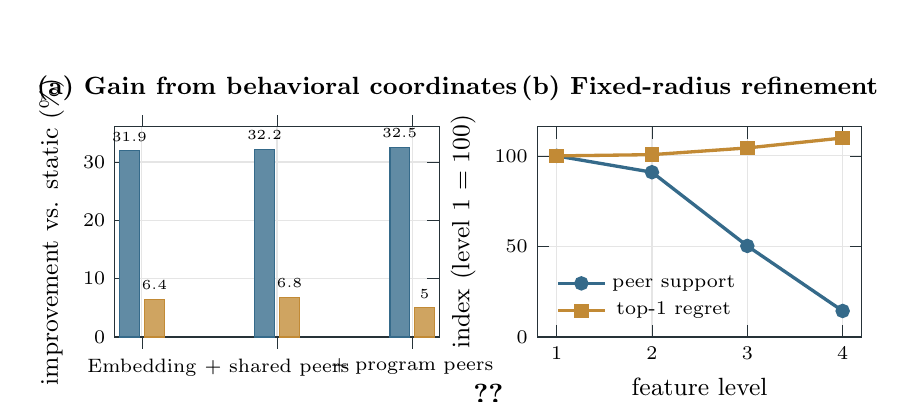
\begin{tikzpicture}
\begin{groupplot}[
  group style={group size=2 by 1,horizontal sep=1.25cm},
  width=.47\linewidth,
  height=4.25cm,
  axis line style={draw=ink},
  tick style={draw=ink},
  tick label style={font=\scriptsize},
  label style={font=\small},
  title style={font=\small\bfseries},
  legend style={font=\scriptsize,draw=none,fill=none},
  grid=major,
  grid style={draw=black!10}
]
\nextgroupplot[
  title={(a) Gain from behavioral coordinates},
  ybar,
  bar width=7pt,
  ymin=0,ymax=36,
  ylabel={improvement vs. static (\%)},
  symbolic x coords={Embedding,Shared,Program},
  xtick=data,
  xticklabels={Embedding,$+$ shared peers,$+$ program peers},
  x tick label style={font=\scriptsize,align=center},
  nodes near coords,
  nodes near coords style={font=\tiny,/pgf/number format/fixed,/pgf/number format/precision=1},
  legend columns=2,
  legend to name=experimentlegend
]
\addplot[fill=blue!78,draw=blue] coordinates
  {(Embedding,31.9) (Shared,32.2) (Program,32.5)};
\addplot[fill=gold!78,draw=gold] coordinates
  {(Embedding,6.4) (Shared,6.8) (Program,5.0)};
\legend{RMSE reduction,Regret reduction}

\nextgroupplot[
  title={(b) Fixed-radius refinement},
  xmin=.8,xmax=4.2,
  ymin=0,ymax=116,
  xtick={1,2,3,4},
  xlabel={feature level},
  ylabel={index (level 1 $=100$)},
  legend pos=south west
]
\addplot[blue,very thick,mark=*,mark options={fill=blue}] coordinates
  {(1,100) (2,91.0) (3,50.3) (4,14.4)};
\addplot[gold,very thick,mark=square*,mark options={fill=gold}] coordinates
  {(1,100) (2,100.7) (3,104.4) (4,109.9)};
\legend{peer support,top-1 regret}
\end{groupplot}
\node at ($(group c1r1.south east)!.5!(group c2r1.south west)+(0,-.72cm)$)
  {\ref{experimentlegend}};
\end{tikzpicture}
\refstepcounter{figure}
\parbox{.95\linewidth}{\small\textbf{Figure \thefigure.} \textbf{Experimental geometry.} Panel (a) reports percentage improvements over the static propensity model in the ten-split chronological experiment; positive values are better. Panel (b) indexes the first pilot's fixed-radius support and regret to level 1. Added feature blocks remove peers rapidly, and recommendation regret rises once refinement outruns support.}
\label{fig:experiments}
\end{center}

\section{Interpretation and scope}

The empirical and theoretical results play different roles. Behavioral embeddings carry most of the predictive gain, while propensity neighborhoods provide a smaller local calibration layer. The operational experiment finds a consistent RMSE improvement but no detectable change in the winning recommendation, and its valid realized-outcome certificate is not sharper than conformal calibration of the base model. The theorem does not presume that every refinement helps: its contribution is a finite-sample regret guarantee that exposes the price of asking for a closer match, while Corollary~\ref{cor:operational} states exactly what additional residual information makes that guarantee computable at test time.

That information can range from a modeled band to exact domain knowledge. When a coordinate is deterministically known---for example, current enrollment makes its propensity one---Remark~\ref{rem:known} removes uncertainty for that coordinate. When propensities remain latent, the band in Corollary~\ref{cor:operational} is an explicit assumption to be justified by the data-generating design. When only exchangeable held-out outcomes are available, \eqref{eq:conformal-operational} provides finite-sample marginal coverage for those outcomes, not a pointwise guarantee for the conditional propensity. Keeping these regimes separate is essential to the interpretation of the theory and experiments.

Enrollment propensity and causal value answer different questions. The present result concerns enrollment propensity. If the objective is incremental enrollment or energy savings, $p_a(x)$ can be replaced by an identified action-specific treatment effect under the corresponding assignment and policy-evaluation design \cite{dudik}. Foundational utility evidence shows that customer targeting can materially affect program savings and cost effectiveness \cite{jones}. Recent work uses causal forests to target household energy interventions \cite{knittel} and machine learning to direct retrofit funds toward projects with higher predicted net benefits \cite{christensen}. Those studies optimize heterogeneous causal or economic returns; this note instead studies enrollment choice and the reliability of a local propensity correction, while leaving the same workflow open to identified treatment-effect targets.

The propositions say exactly what refinement does, and the theorem prices what it costs. The embedding and propensity matrix show where the method fits in a working recommender. Together, these pieces form an end-to-end workflow from eligibility and behavioral representation through propensity scoring and support-aware calibration to a certified recommendation or abstention. The argument therefore closes with the same three claims with which it began:

\begin{center}
\emph{Behavioral embeddings provide the largest empirical gain by creating customer coordinates that preserve future propensity similarity. Operational peer-mean neighborhood calibration adds a small but consistent improvement in propensity RMSE, without a detectable improvement in the winning recommendation. The refinement-frontier theorem and its operational corollaries provide finite-sample guarantees for latent propensities under a valid residual band and marginal guarantees for realized outcomes under exchangeability.}
\end{center}

\begin{thebibliography}{18}\scriptsize
\setlength{\itemsep}{.12ex}
\setlength{\parskip}{0pt}

\bibitem{koren}
Y. Koren, R. Bell, and C. Volinsky, ``Matrix factorization techniques for recommender systems,'' \emph{Computer}, 42(8):30--37, 2009.

\bibitem{sasrec}
W.-C. Kang and J. McAuley, ``Self-attentive sequential recommendation,'' in \emph{Proc. IEEE ICDM}, pp. 197--206, 2018.

\bibitem{bert4rec}
F. Sun, J. Liu, J. Wu, C. Pei, X. Lin, W. Ou, and P. Jiang, ``BERT4Rec: Sequential recommendation with bidirectional encoder representations from Transformer,'' in \emph{Proc. ACM CIKM}, pp. 1441--1450, 2019.

\bibitem{tiger}
S. Rajput, N. Mehta, A. Singh, R. H. Keshavan, T. Vu, L. Heldt, L. Hong, Y. Tay, V. Q. Tran, J. Samost, M. Kula, E. H. Chi, and M. Sathiamoorthy, ``Recommender systems with generative retrieval,'' in \emph{Advances in Neural Information Processing Systems}, vol. 36, 2023.

\bibitem{stone}
C. J. Stone, ``Consistent nonparametric regression,'' \emph{Annals of Statistics}, 5(4):595--620, 1977.

\bibitem{luo}
R. Luo, A. Bhatnagar, Y. Bai, S. Zhao, H. Wang, C. Xiong, S. Savarese, S. Ermon, E. Schmerling, and M. Pavone, ``Local calibration: Metrics and recalibration,'' in \emph{Proc. UAI}, PMLR 180:1286--1295, 2022.

\bibitem{hoeffding}
W. Hoeffding, ``Probability inequalities for sums of bounded random variables,'' \emph{Journal of the American Statistical Association}, 58(301):13--30, 1963.

\bibitem{shafer}
G. Shafer and V. Vovk, ``A tutorial on conformal prediction,'' \emph{Journal of Machine Learning Research}, 9:371--421, 2008.

\bibitem{guo}
C. Guo, G. Pleiss, Y. Sun, and K. Q. Weinberger, ``On calibration of modern neural networks,'' in \emph{Proc. ICML}, PMLR 70:1321--1330, 2017.

\bibitem{venn}
L. Van Der Laan and A. Alaa, ``Generalized Venn and Venn--Abers calibration with applications in conformal prediction,'' in \emph{Proc. ICML}, PMLR 267:60748--60763, 2025.

\bibitem{covington}
P. Covington, J. Adams, and E. Sargin, ``Deep neural networks for YouTube recommendations,'' in \emph{Proc. ACM Conference on Recommender Systems}, pp. 191--198, 2016.

\bibitem{zhangplan}
Y. Zhang, K. Meng, W. Kong, and Z. Y. Dong, ``Collaborative filtering-based electricity plan recommender system,'' \emph{IEEE Transactions on Industrial Informatics}, 15(3):1393--1404, 2019.

\bibitem{liang}
H. Liang, J. Ma, R. Sun, and Y. Du, ``A data-driven approach for targeting residential customers for energy efficiency programs,'' \emph{IEEE Transactions on Smart Grid}, 11(2):1229--1238, 2020.

\bibitem{gao}
C. Gao, S. Li, W. Lei, J. Chen, B. Li, P. Jiang, X. He, J. Mao, and T.-S. Chua, ``KuaiRec: A Fully-Observed Dataset and Insights for Evaluating Recommender Systems,'' in \emph{Proc. CIKM}, pp. 540--550, 2022.

\bibitem{dudik}
M. Dud\'{i}k, J. Langford, and L. Li, ``Doubly robust policy evaluation and learning,'' in \emph{Proc. ICML}, pp. 1097--1104, 2011.

\bibitem{jones}
N. W. Taylor, P. H. Jones, and M. J. Kipp, ``Targeting utility customers to improve energy savings from conservation and efficiency programs,'' \emph{Applied Energy}, 115:25--36, 2014.

\bibitem{knittel}
C. R. Knittel and S. Stolper, ``Using machine learning to target treatment: The case of household energy use,'' \emph{Economic Journal}, 135(672):2377--2401, 2025.

\bibitem{christensen}
P. Christensen, P. Francisco, E. Myers, H. Shao, and M. Souza, ``Energy efficiency can deliver for climate policy: Evidence from machine learning-based targeting,'' \emph{Journal of Public Economics}, 234:105098, 2024.

\end{thebibliography}

\end{document}
